\documentclass[12pt,a4paper,portrait]{article}
%\setcounter{secnumdepth}{0}
\usepackage{gensymb}
\usepackage{pdflscape}
\usepackage{amsmath}
\usepackage{amssymb}
\usepackage{enumitem}
\usepackage{graphicx}
\usepackage{subcaption}
\usepackage{multirow}
\usepackage{sansmath}
\usepackage{pst-eucl}
\usepackage{multicol}
\usepackage{csquotes}
% Coding
\usepackage{listings}
\setlength{\parindent}{0pt}
\usepackage[obeyspaces]{url}
% Better inline directory listings
\usepackage{xcolor}
\definecolor{light-gray}{gray}{0.95}
\newcommand{\code}[1]{\colorbox{light-gray}{\texttt{#1}}}
\usepackage{adjustbox}
\usepackage[UKenglish]{isodate}
\usepackage[UKenglish]{babel}
\usepackage{float}
\usepackage[T1]{fontenc}
\usepackage{setspace}
\usepackage{sectsty}
\usepackage{longtable}
\newenvironment{tightcenter}{%
	\setlength\topsep{0pt}
	\setlength\parskip{0pt}
	\begin{center}
	}{%
	\end{center}
}
\captionsetup{width=\textwidth}
\usepackage{mbenotes} % to print table notes!
\usepackage{alphalph} % For extended counters!
% usage: \tabnotemark[3]\cmsp\tabnotemark[4]
\usepackage[colorlinks=true,linkcolor=blue,urlcolor=black,bookmarksopen=true]{hyperref}
\sectionfont{%			            % Change font of \section command
	\usefont{OT1}{phv}{b}{n}%		% bch-b-n: CharterBT-Bold font
	\sectionrule{0pt}{0pt}{-5pt}{3pt}}
\subsectionfont{
	\usefont{OT1}{phv}{b}{n}}
\newcommand{\MyName}[1]{ % Name
	\usefont{OT1}{phv}{b}{n} \begin{center}of {\LARGE  #1}\end{center}
	\par \normalsize \normalfont}
\makeatletter
\newcommand\FirstWord[1]{\@firstword#1 \@nil}%
\newcommand\@firstword{}%
\newcommand\@removecomma{}%
\def\@firstword#1 #2\@nil{\@removecomma#1,\@nil}%
\def\@removecomma#1,#2\@nil{#1}
\makeatother

\newcommand{\MyTitle}[1]{ % Name
	\Huge \usefont{OT1}{phv}{b}{n} \begin{center}#1\end{center}
	\par \normalsize \normalfont}
\newcommand{\NewPart}[1]{\section*{\uppercase{#1}}}
\newcommand{\NewSubPart}[1]{\subsection*{\hspace{0.2cm}#1}}
\renewcommand{\baselinestretch}{1.05}
\usepackage[margin=0.2cm]{geometry}
\date{}
\title{Elastic pendulums}
\author{Brenton Horne}

\begin{document}
\maketitle

\tableofcontents

\section{Single elastic pendulum with friction}
Say we have a mass $m$ attached to a spring of rest length $l_0$. Suppose we call the displacement from rest $z$. That way the length of the spring is $l(t) = l_0 + z$. Let us measure  $\theta$ clockwise from the positive x-axis.

\subsection{Position and velocity}
Cartesian coordinates are defined as:

\begin{align*}
	x &= (l_0+z)\cos{\theta} &\implies \dot{x} &= \dot{z}\cos{\theta} - (l_0+z)\dot{\theta}\sin{\theta}\\
	y &= (l_0+z)\sin{\theta} &\implies \dot{y} &= \dot{z}\sin{\theta} + (l_0+z)\dot{\theta}\cos{\theta}.\\
\end{align*}

Velocity is given by:

\begin{align*}
	\vec{v} &= \begin{bmatrix}
		\dot{z}\cos{\theta} - (l_0+z)\dot{\theta}\sin{\theta} \\
		\dot{z}\sin{\theta} + (l_0+z)\dot{\theta}\cos{\theta}
	\end{bmatrix}\\
	v^2 &= |\vec{v}|^2 \\
	&= \dot{x}^2+\dot{y}^2 \\
	&= \left[\dot{z}\cos{\theta} - (l_0+z)\dot{\theta}\sin{\theta}\right]^2 + \left[\dot{z}\sin{\theta} + (l_0+z)\dot{\theta}\cos{\theta}\right]^2 \\
	&= \dot{z}^2 \cos^2{\theta} + (l_0+z)^2\dot{\theta}^2\sin^2{\theta} - 2\dot{z}\dot{\theta}(l_0+z)\cos{\theta}\sin{\theta} + \dot{z}^2\sin^2{\theta} + (l_0+z)^2\dot{\theta}^2\cos^2{\theta} + 2\dot{z}\dot{\theta}(l_0+z)\sin{\theta}\cos{\theta} \\
	&= \dot{z}^2 + (l_0+z)^2\dot{\theta}^2\\
\therefore |\vec{v}| &= \sqrt{v^2}\\
	&= \sqrt{\dot{z}^2+(l_0+z)^2\dot{\theta}^2}.
\end{align*}

\subsection{Generalized basis vector}
Next we will calculate $\dfrac{\partial \vec{r}}{\partial q_i}$:

\begin{align*}
	\dfrac{\partial \vec{r}}{\partial \theta} &= (l_0+z)\begin{bmatrix}
		-\sin{\theta} \\
		\cos{\theta}
	\end{bmatrix} \\
	\dfrac{\partial \vec{r}}{\partial z} &= \begin{bmatrix}
		\cos{\theta} \\
		\sin{\theta}
	\end{bmatrix}.
\end{align*}

\subsection{Kinetic energy}
Hence the kinetic energy is:
\begin{align*}
	T &= \dfrac{mv^2}{2} \\
	&= \dfrac{m}{2} \left[\dot{z}^2 + (l_0+z)^2\dot{\theta}^2\right].
\end{align*}

\subsection{Potential energy}
As for the potential energy, it will have two components: a spring component,
\begin{align*}
	V_S &= \dfrac{kz^2}{2};
\end{align*}

and a graphical component,
\begin{align*}
	V_G &= mgy \\
	&= mg(l_0+z)\sin{\theta}.
\end{align*}

Therefore the total potential energy is:
\begin{align*}
	V &= V_S + V_G \\
	&= \dfrac{kz^2}{2} + mg(l_0+z)\sin{\theta}.
\end{align*}

\subsection{Lagrangian}
Hence the Lagrangian is:
\begin{align*}
	\mathcal{L} &= T - V \\
	&= \dfrac{m}{2} \left[\dot{z}^2 + \dot{\theta}^2(l_0+z)^2\right] - \dfrac{kz^2}{2} - mg(l_0+z)\sin{\theta}.
\end{align*}

\subsection{Equations of motion}
To find the equations of motion, we use the Euler-Lagrange equations with a dissipative force:
\begin{align}
	\dfrac{d}{dt}\left(\dfrac{\partial \mathcal{L}}{\partial \dot{q}_i}\right) - \dfrac{\partial \mathcal{L}}{\partial q_i} &= Q_i. \label{ELD}
\end{align}

Where $Q_i$ is the generalized dissipative force calculated using:
\begin{align*}
	Q_i &= \vec{F}_{D} \cdot \dfrac{\partial \vec{r}}{\partial q_i}.
\end{align*}

$\vec{F}_D$ is the dissipative force. In this case, our generalized coordinates $q_i$ would consist of $\theta$ and $z$. 

\subsection{Dissipative forces}
What dissipative forces should be included? Let us include linear and quadratic in velocity terms to account for air resistance and other forms of friction. 

\begin{align*}
	\vec{F}_D &= -b\vec{v} - c|\vec{v}|\vec{v}.
\end{align*}

We have already calculate the components of the velocity vector---they are $\dot{x}$ and $\dot{y}$, respectively. 

\begin{align*}
	\vec{v} &= \begin{bmatrix}
		\dot{z}\cos{\theta} - (l_0+z)\dot{\theta}\sin{\theta} \\
		\dot{z}\sin{\theta} + (l_0+z)\dot{\theta}\cos{\theta}
	\end{bmatrix}\\
	|\vec{v}| &= \sqrt{v^2}\\
	&= \sqrt{\dot{z}^2+(l_0+z)^2\dot{\theta}^2}.
\end{align*}

To calculate, $Q_i$ we must find $\vec{v} \cdot \dfrac{\partial \vec{r}}{\partial q_i}$:

\begin{align*}
	\vec{v} \cdot \dfrac{\partial \vec{r}}{\partial \theta} &= \begin{bmatrix}
		\dot{z}\cos{\theta} - (l_0+z)\dot{\theta}\sin{\theta} \\
		\dot{z}\sin{\theta} + (l_0+z)\dot{\theta}\cos{\theta}
	\end{bmatrix} \cdot (l_0+z)\begin{bmatrix}
		-\sin{\theta} \\
		\cos{\theta}
	\end{bmatrix} \\
	&= -\dot{z}(l_0+z)\cos{\theta} \sin{\theta} + (l_0+z)^2 \dot{\theta}\sin^2{\theta} + \dot{z}(l_0+z)\sin{\theta} \cos{\theta} +(l_0+z)^2\dot{\theta}\cos^2{\theta} \\
	&= (l_0+z)^2 \dot{\theta} \\
	\vec{v} \cdot \dfrac{\partial \vec{r}}{\partial z} &= \begin{bmatrix}
		\dot{z}\cos{\theta} - (l_0+z)\dot{\theta}\sin{\theta} \\
		\dot{z}\sin{\theta} + (l_0+z)\dot{\theta}\cos{\theta}
	\end{bmatrix} \cdot \begin{bmatrix}
		\cos{\theta} \\
		\sin{\theta}
	\end{bmatrix} \\
	&= \dot{z}\cos^2{\theta} - (l_0+z)\dot{\theta} \sin{\theta}\cos{\theta} + \dot{z}\sin^2{\theta} + (l_0+z)\dot{\theta}\cos{\theta}\sin{\theta} \\
	&= \dot{z}. 
\end{align*}

Hence $Q_i$ is:

\begin{align*}
	Q_{\theta} &= -(l_0+z)^2 \dot{\theta} \left(b+c\sqrt{\dot{z}^2+(l_0+z)^2\dot{\theta}^2}\right) \\
	Q_z &= -\dot{z}\left(b+c\sqrt{\dot{z}^2+(l_0+z)^2\dot{\theta}^2}\right).
\end{align*}

\subsection{Left-hand side of Equation \eqref{ELD}}
\subsubsection{$\theta$}
As for the LHS of Equation \eqref{ELD}, let us work on it for $\theta$ one term at a time:
\begin{align*}
	p_{\theta} &= \dfrac{\partial \mathcal{L}}{\partial \dot{\theta}} \\
	&= m\dot{\theta}(l_0+z)^2 \\
	\dot{p_{\theta}} &= m\ddot{\theta} (l_0+z)^2 + 2m\dot{\theta}\dot{z}(l_0+z) \\
	F_{\theta} &= \dfrac{\partial \mathcal{L}}{\partial \theta} \\
	&= -mg(l_0+z)\cos{\theta}.
\end{align*}

Substituting into Equation \eqref{ELD} yields:
\begin{align*}
	m\ddot{\theta} (l_0+z)^2 + 2m\dot{\theta}\dot{z}(l_0+z) - (-mg(l_0+z)\cos{\theta}) &= -(l_0+z)^2 \dot{\theta} \left(b+c\sqrt{\dot{z}^2+(l_0+z)^2\dot{\theta}^2}\right) \\
	m\ddot{\theta} (l_0+z)^2 + 2m\dot{\theta}\dot{z}(l_0+z) +mg(l_0+z)\cos{\theta} &= -(l_0+z)^2 \dot{\theta} \left(b+c\sqrt{\dot{z}^2+(l_0+z)^2\dot{\theta}^2}\right) \\
	\ddot{\theta} &= -\dfrac{2\dot{\theta}\dot{z}}{l_0+z} - \dfrac{g\cos{\theta}}{l_0+z} -\dfrac{\dot{\theta}}{m} \left(b+c\sqrt{\dot{z}^2+(l_0+z)^2\dot{\theta}^2}\right). \\
\end{align*}

Let $k'=\dfrac{k}{m}$, $b'=\dfrac{b}{m}$ and $c'=\dfrac{c}{m}$.

\begin{align*}
	\ddot{\theta} &= -\dfrac{2\dot{\theta}\dot{z}}{l_0+z} - \dfrac{g\cos{\theta}}{l_0+z} -\dot{\theta} \left(b'+c'\sqrt{\dot{z}^2+(l_0+z)^2\dot{\theta}^2}\right).
\end{align*}

\subsubsection{$z$}
As for $z$:

\begin{align*}
	p_z &= \dfrac{\partial \mathcal{L}}{\partial \dot{z}} \\
	&= m\dot{z} \\
	\dot{p_z} &= m\ddot{z} \\
	F_z &= \dfrac{\partial \mathcal{L}}{\partial z} \\
	&= m\dot{\theta}^2(l_0+z) - kz - mg\sin{\theta}.
\end{align*}

Substituting into Equation \eqref{ELD} yields:

\begin{align*}
	m\ddot{z} - m\dot{\theta}^2(l_0+z) + kz + mg\sin{\theta} &= -\dot{z}\left(b+c\sqrt{\dot{z}^2+(l_0+z)^2\dot{\theta}^2}\right) \\
	\ddot{z} &= \dot{\theta}^2(l_0+z) - \dfrac{kz}{m} - g\sin{\theta} -\dfrac{\dot{z}}{m}\left(b+c\sqrt{\dot{z}^2+(l_0+z)^2\dot{\theta}^2}\right).
\end{align*}

Let $k'=\dfrac{k}{m}$, $b'=\dfrac{b}{m}$ and $c'=\dfrac{c}{m}$.

\begin{align*}
	\ddot{z} &= \dot{\theta}^2(l_0+z) - k'z - g\sin{\theta} -\dot{z}\left(b'+c'\sqrt{\dot{z}^2+(l_0+z)^2\dot{\theta}^2}\right).
\end{align*}


\section{Double pendulum with an elastic second pendulum}
Below we will analyse the double pendulum where the second pendulum is elastic. The rest length of the elastic pendulum is $l$ and its displacement from rest is $x$. Let the masses of the pendulum bobs be $m_1$ and $m_2$, respectively. We will assume the rod/string have no mass. I have tried accounting for it, using a centre of mass approach, in my double pendulum calculation and my experience with simulations is that it does not really make things any more interesting and just adds complexity. 
\begin{figure}[H]
	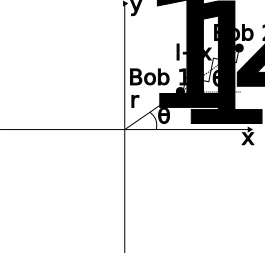
\includegraphics[width=300px]{Double pendulum second elastic.png}
\end{figure}

\subsection{Positions and velocities}
\begin{align*}
	x_1 &= r_1 \cos{\theta_1} &\therefore \dot{x}_1 &= -r_1 \dot{\theta}_1 \sin{\theta_1}\\
	y_1 &= r_1 \sin{\theta_1} &\therefore \dot{y}_1 &= r_1 \dot{\theta}_1 \cos{\theta_1} \\
	x_2 &= x_1 + (l_0+z)\cos{\theta_2} & \therefore v_1^2 &= r_1^2 \dot{\theta}_1^2\\
	&= r_1 \cos{\theta_1} + (l_0+z)\cos{\theta_2} &\therefore \dot{x}_2 &= -r_1 \dot{\theta}_1 \sin{\theta_1} + \dot{z} \cos{\theta_2}-(l_0+z)\dot{\theta}_2 \sin{\theta_2}\\
	y_2 &= y_1 + (l_0+z)\sin{\theta_2} \\
	&= r_1\sin{\theta_1} + (l_0+z)\sin{\theta_2} &\therefore \dot{y}_2 &= r_1 \dot{\theta}_1 \cos{\theta_1} + \dot{z} \sin{\theta_2}+(l_0+z)\dot{\theta}_2 \cos{\theta_2}
\end{align*}
\begin{align*}
	v_2^2 &= \left( -r_1 \dot{\theta}_1 \sin{\theta_1} + \dot{z} \cos{\theta_2}-(l_0+z)\dot{\theta}_2 \sin{\theta_2}\right)^2 + \left(r_1 \dot{\theta}_1 \cos{\theta_1} + \dot{z} \sin{\theta_2}+(l_0+z)\dot{\theta}_2 \cos{\theta_2}\right)^2 \\
	&= r_1^2 \dot{\theta}_1^2 \sin^2{\theta_1}+\dot{z}^2 \cos^2{\theta_2}+(l_0+z)^2 \dot{\theta}_2^2 \sin^2{\theta_2} - 2r_1 \dot{\theta}_1 \dot{z}\sin{\theta_1}\cos{\theta_2} + 2r_1 (l_0+z)\dot{\theta}_1 \dot{\theta}_2 \sin{\theta_1}\sin{\theta_2}\\
	&-2\dot{z}(l_0+z)\dot{\theta}_2 \cos{\theta_2}\sin{\theta_2}+r_1^2\dot{\theta}_1^2 \cos^2{\theta_1} + \dot{z}^2 \sin^2{\theta_2} + (l_0+z)^2 \dot{\theta}_2^2\cos^2{\theta_2} + 2r_1(l_0+z)\dot{\theta}_1\dot{\theta}_2\cos{\theta_1}\cos{\theta_2}\\
	&+2r_1\dot{z}\dot{\theta}_1 \cos{\theta_1}\sin{\theta_2}+2\dot{z}\dot{\theta}_2(l_0+z)\sin{\theta_2}\cos{\theta_2} \\
	&= r_1^2 \dot{\theta}_1^2 + \dot{z}^2 + (l_0+z)^2\dot{\theta}_2^2 + 2r_1\dot{\theta}_1 \dot{z} (\cos{\theta_1}\sin{\theta_2} - \sin{\theta_1}\cos{\theta_2}) + 2r_1(l_0+z)\dot{\theta}_1\dot{\theta}_2(\sin{\theta_1}\sin{\theta_2} + \cos{\theta_1}\cos{\theta_2})\\
	&+2\dot{z}\dot{\theta}_2(l_0+z)(\sin{\theta_2}\cos{\theta_2}-\sin{\theta_2}\cos{\theta_2})
\end{align*}
\begin{align*}
	v_2^2 &= r_1^2 \dot{\theta}_1^2 + \dot{z}^2 + (l_0+z)^2\dot{\theta}_2^2 + 2r_1\dot{\theta}_1 \dot{z} \sin{(\theta_2-\theta_1)} + 2r_1(l_0+z)\dot{\theta}_1\dot{\theta}_2\cos{(\theta_2 - \theta_1)}.
\end{align*}
\subsection{Generalized basis vectors}
\begin{align*}
	\dfrac{\partial \vec{r}_1}{\partial \theta_1} &= r_1\begin{bmatrix}
		-\sin{\theta_1} \\
		\cos{\theta_1}
	\end{bmatrix} & \dfrac{\partial \vec{r}_1}{\partial \theta_2} &= \dfrac{\partial \vec{r}_1}{\partial z} \\
	\dfrac{\partial \vec{r}_2}{\partial \theta_1} &= r_1\begin{bmatrix}
		-\sin{\theta_1} \\
		\cos{\theta_1}
	\end{bmatrix} & &= 0. \\
	\dfrac{\partial \vec{r}_2}{\partial \theta_2} &= (l_0+z)\begin{bmatrix}
		-\sin{\theta_2} \\
		\cos{\theta_2}
	\end{bmatrix} & \dfrac{\partial \vec{r}_2}{\partial z} &= \begin{bmatrix}
		\cos{\theta_2}\\
		\sin{\theta_2}
	\end{bmatrix}.
\end{align*}

\subsection{Kinetic energy}
\begin{align*}
	T &= \dfrac{m_1}{2}v_1^2 + \dfrac{m_2}{2}v_2^2 \\
	&= \dfrac{m_1r_1^2 \dot{\theta}_1^2}{2} + \dfrac{m_2(r_1^2 \dot{\theta}_1^2 + \dot{z}^2 + (l_0+z)^2\dot{\theta}_2^2 + 2r_1\dot{\theta}_1 \dot{z} \sin{(\theta_2-\theta_1)} + 2r_1(l_0+z)\dot{\theta}_1\dot{\theta}_2\cos{(\theta_2 - \theta_1)})}{2}\\
	&= \dfrac{m_1+m_2}{2}r_1^2\dot{\theta}_1^2 + \dfrac{m_2(\dot{z}^2 + (l_0+z)^2\dot{\theta}_2^2 + 2r_1\dot{\theta}_1[ \dot{z} \sin{(\theta_2-\theta_1)} + (l_0+z)\dot{\theta}_2\cos{(\theta_2 - \theta_1)}])}{2}.
\end{align*}

\subsection{Potential energy}
\subsubsection{First bob}
For the first bob, the only potential energy is gravitational. 
\begin{align*}
	V_1 &= m_1gy_1 \\
	&= m_1 gr_1\sin{\theta_1}.
\end{align*}

\subsubsection{Second bob}
For the second bob, there is the spring potential energy and the gravitational potential energy to consider:

\begin{align*}
	V_2 &= m_2gy_2 + \dfrac{kz^2}{2} \\
	&= m_2 g(r_1\sin{\theta_1} + (l_0+z)\sin{\theta_2}) + \dfrac{kz^2}{2}.
\end{align*}

\subsubsection{Total}
The total potential energy is therefore:

\begin{align*}
	V &= V_1 + V_2 \\
	&= m_1 gr_1\sin{\theta_1} + m_2 g(r_1\sin{\theta_1} + (l_0+z)\sin{\theta_2}) + \dfrac{kz^2}{2}.
\end{align*}

\subsection{Lagrangian}
\begin{align*}
	\mathcal{L} &= T - V \\
	&= \dfrac{m_1+m_2}{2}r_1^2\dot{\theta}_1^2 + \dfrac{m_2(\dot{z}^2 + (l_0+z)^2\dot{\theta}_2^2 + 2r_1\dot{\theta}_1[ \dot{z} \sin{(\theta_2-\theta_1)} + (l_0+z)\dot{\theta}_2\cos{(\theta_2 - \theta_1)}])}{2} - m_1 gr_1\sin{\theta_1} \\
	&- m_2 g(r_1\sin{\theta_1} + (l_0+z)\sin{\theta_2}) - \dfrac{kz^2}{2}.
\end{align*}

\subsection{Euler-Lagrange equations}
\begin{align*}
	p_{\theta_1} &= \dfrac{\partial \mathcal{L}}{\partial \dot{\theta}_1} \\
	&= (m_1+m_2)r_1^2 \dot{\theta}_1 + m_2r_1[ \dot{z} \sin{(\theta_2-\theta_1)} + (l_0+z)\dot{\theta}_2\cos{(\theta_2 - \theta_1)}] \\
	\dot{p}_{\theta_1} &= (m_1+m_2)r_1^2 \ddot{\theta}_1 +  m_2r_1[ \ddot{z} \sin{(\theta_2-\theta_1)} + \dot{z}(\dot{\theta}_2-\dot{\theta}_1)\cos{(\theta_2-\theta_1)}+ (l_0+z)\ddot{\theta}_2\cos{(\theta_2 - \theta_1)} \\
	&- (l_0+z)\dot{\theta}_2(\dot{\theta}_2-\dot{\theta}_1)\sin{(\theta_2 - \theta_1)}+\dot{z}\dot{\theta}_2\cos{(\theta_2 - \theta_1)}]\\
	&= (m_1+m_2)r_1^2 \ddot{\theta}_1 +  m_2r_1[(\ddot{z} -(l_0+z)\dot{\theta}_2(\dot{\theta}_2-\dot{\theta}_1))\sin{(\theta_2 - \theta_1)}+(\dot{z}(2\dot{\theta}_2-\dot{\theta}_1)+(l_0+z)\ddot{\theta}_2)\cos{(\theta_2-\theta_1)}]
\end{align*}

Calculating the generalized force for $\theta_1$ (a term taken from \href{https://phys.libretexts.org/Bookshelves/Classical_Mechanics/Graduate_Classical_Mechanics_(Fowler)/04%3A_Hamilton's_Principle_and_Noether's_Theorem/4.05%3A_Generalized_Momenta_and_Forces}{Fowler's Graduate Classical Mechanics})
\begin{align*}
	 F_{\theta_1} &= \dfrac{\partial \mathcal{L}}{\partial \theta_1} \\
	 &= m_2 r_1 \dot{\theta}_1(\dot{z}\cos{(\theta_2-\theta_1)}\cdot -1 -(l_0+z)\dot{\theta}_2 \sin{(\theta_2-\theta_1)}\cdot -1) - m_1gr_1 \cos{\theta_1} - m_2gr_1\cos{\theta_1} \\
	 &= m_2 r_1\dot{\theta}_1((l_0+z)\dot{\theta}_2 \sin{(\theta_2-\theta_1)}-\dot{z}\cos{(\theta_2-\theta_1)}) -(m_1+m_2)gr_1\cos{\theta_1}
\end{align*}
\end{document}